\chapter{Introduction and Motivation}
A sensor is an analytical device designed to detect and respond to a 
specific input stimulus from the physical environment, translating it 
into a measurable analog or digital signal. These input stimuli encompass 
a vast array of environmental phenomena, such as pressure, force, flow, 
light, heat, motion, or moisture. The resulting output is typically 
converted into an electrical signal that can be subsequently processed, 
measured, and analyzed \cite{javaid2021}.

In order to better understand physical reality, a wide variety of sensors 
have been developed throughout human history, with some of the earliest 
documented mechanisms dating back thousands of years. Early sensing 
principles relied entirely on mechanical, hydraulic, and pneumatic 
feedback loops rather than electronic transduction. For instance, 
Heron of Alexandria developed an automatic mechanism for opening and 
closing temple doors in 62 CE. This device utilized the thermal 
expansion of air to trigger mechanical motion, as illustrated in 
Figure~\ref{fig:herondoor}. Similarly, Zhang Heng's seismoscope 
(132 CE) employed an inertia-based internal pendulum to detect and 
indicate the direction of distant earthquakes, as detailed in 
Figure~\ref{fig:seismoscope}.
\begin{figure}[h]
    \centering
    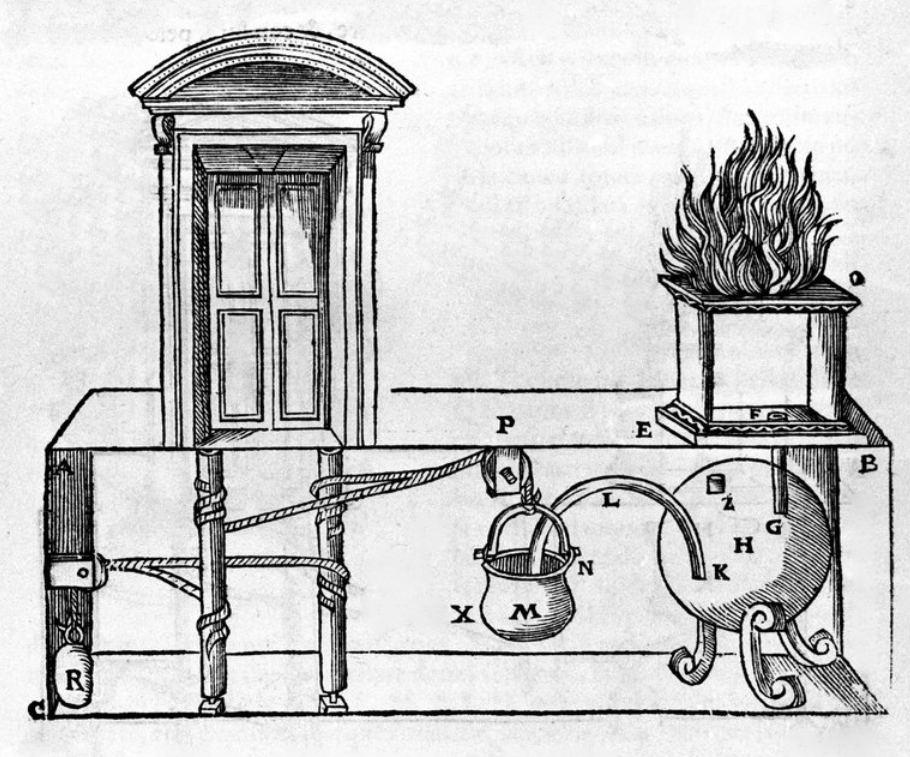
\includegraphics[width=0.75\linewidth]{Images/herondoor.png}
    \caption{Automatic mechanism for temple door actuation designed by 
    Heron of Alexandria (62 CE). When the altar fire is lit, the air 
    confined within cavity (E) undergoes thermal expansion, increasing 
    the pneumatic pressure inside the water-filled reservoir (H). 
    This pressure forces water through pipe (L) into the suspended 
    cauldron (M). The resulting weight displacement overcomes 
    the counterweight (R), thereby opening the doors. Once the 
    fire is extinguished, pressure drops, and the system reverts 
    to its equilibrium state. Adapted from \cite{herondoor}.}
    \label{fig:herondoor}
\end{figure}
\begin{figure}[h]
    \centering
    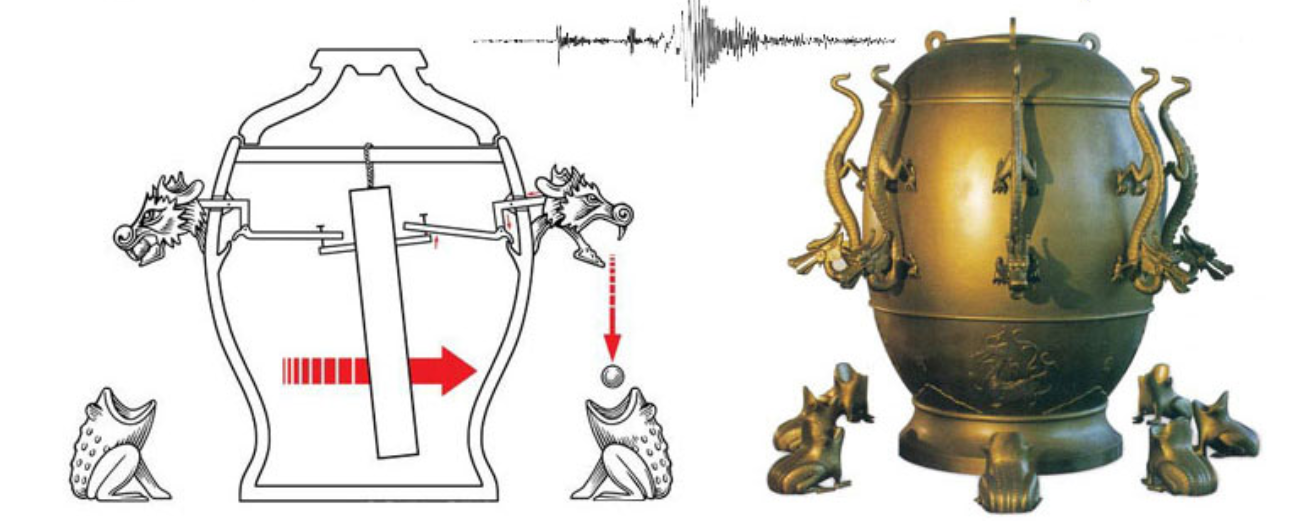
\includegraphics[width=0.75\linewidth]{Images/seismoscope.png}
    \caption{Seismoscope developed by Chinese polymath Zhang Heng (132 CE). 
    A central pendulum suspended inside the bronze vessel oscillates in 
    response to seismic vibrations. This displacement triggers an internal 
    lever mechanism that opens the jaws of a specific dragon head, releasing 
    a bronze ball into the mouth of a corresponding frog statue below. 
    Eight radial dragon-frog pairs were meticulously aligned to determine 
    the primary orientation of the earthquake epicenter. Adapted from \cite{seismoscope}.}
    \label{fig:seismoscope}
\end{figure}

Modern sensors began to emerge during the 17th century. These devices commonly rely 
on three key interconnected elements: (i) a receptor that specifically interacts 
with the target analyte or physical stimulus; (ii) a transducer that responds to 
this interaction by producing a characteristic signal; and (iii) a data-processing 
system that computes the signal into measurable quantities and generates usable data 
\cite{pirzada2023}. As one of the earliest examples of this conceptual framework, 
Galileo Galilei invented the thermoscope, which monitored temperature variations 
through the thermal expansion of air. This qualitative device was subsequently 
improved by Santorio Santorio, who introduced a numerical scale, effectively 
transforming the instrument into the first measurable thermometer \cite{middleton1966}.

During the Industrial Revolution (18th to 19th century), the scientific imperative 
to analyze and optimize machine behavior demanded more diverse and sophisticated 
monitoring tools. It was during this era that the foundational concept of transduction (translating 
a physical phenomenon into an actionable, measurable output) was firmly established. 
Concurrently, essential analytical tools such as the barometer, litmus paper, the 
Davy safety lamp, and early mechanical thermostats were developed to ensure industrial 
safety and process control \cite{pirzada2023, duncan1947}.

The 19th century marked a critical turning point in sensor technology by shifting 
the output medium from purely mechanical displacements toward electrical signals. 
The invention of the galvanometer by Johann Schweigger in 1820 allowed for the 
precise measurement of micro-currents, effectively paving the way for electrical 
instrumentation. Later, in 1880, Pierre and Jacques Curie discovered the piezoelectric 
effect, a breakthrough that enabled the development of piezoelectric sensors capable of 
converting mechanical stress directly into measurable electrical charge \cite{curie1880}.

The mid-20th century witnessed the introduction of solid-state electronic sensors, 
transforming global industries by providing faster, more reliable, and highly accurate
measurements. This era was revolutionized by the invention of the point-contact transistor 
at Bell Labs in 1947, which enabled the development of significantly smaller and more efficient 
electronic components \cite{bardeen1948}. Following World War II, the rapid growth of the 
semiconductor industry allowed sensors to become progressively more compact, efficient, and 
affordable. This technological trajectory was further propelled by the introduction of 
integrated circuits (ICs) in the late 1950s and 1960s, a breakthrough that facilitated 
the micro-miniaturization of devices and enabled the integration of multiple sensing 
functions onto a single silicon substrate \cite{kilby1976}. By the 1960s and 1970s, these 
advanced solid-state sensors became widespread across the aerospace, automotive, and 
telecommunications sectors, ultimately forming the technological backbone of complex, 
modern monitoring and control systems.

\section{Microelectromechanical systems (MEMS)}
Microelectromechanical systems (MEMS) refer to devices that have characteristic length of less than
\SI{1}{\milli\meter} but more than \SI{1}{\micro\meter}, that combine electrical and mechanical components, 
and that are fabricated
using integrated circuit batch-processing technologies \cite{memshandbook}. In recent decades,
these technologies have evolved to a wide number of applications thanks to the advantatges 
it presents, such as 1) the
active material, silicon, is abundant, inexpensive, and can now
be produced and processed controllably to unparalleled stan-
dards of purity and perfection; 2) silicon processing itself is
based on very thin deposited films which are highly amenable
to miniaturization; 3) definition and reproduction of the
device shapes and patterns are performed using photographic
techniques which have also, historically, been capable of high
precision and amenable to miniaturization; finally, and most
important of all from a commercial and practical point of
view, 4) silicon microelectronic circuits are batch-fabricated.
The unit of production for integrated circuits-the wafer-is
not one individual saleable item, but contains hundreds of
identical chips \cite{petersen1982}. The high purity and crystalline perfection of available
silicon is expected to optimize the mechanical properties of
devices made from silicon in the same way that electronic
properties have been optimized to increase the performance,
reliability, and reproducibility of device characteristics. 
\begin{figure}[h]
    \centering
    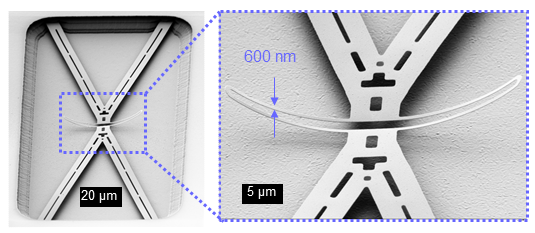
\includegraphics[width=0.75\linewidth]{Images/memspic.png}
    \caption{From \cite{birkholz2013}.}
    \label{fig:scaleofthings}
\end{figure}